%!TEX root = ../Demo.tex
\chapter{自动机状态转移图}

%%  接受{$\mathcal{L}$}=0*10*的自动机{\cite[fig 5-4]{book1}}

\begin{figure}[!htbp]
    \centering
    \begin{subfigure}[b]{0.35\textwidth}
        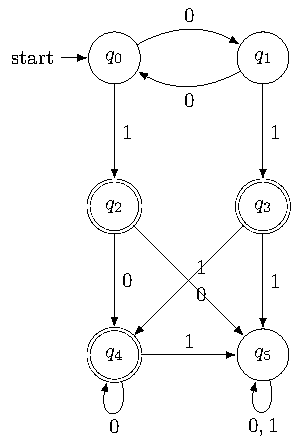
\includegraphics[width=\textwidth]{automaton_4_0}
        \caption{}
        \label{fig:DFA4_0}
    \end{subfigure}
    ~
    \begin{subfigure}[b]{0.35\textwidth}
        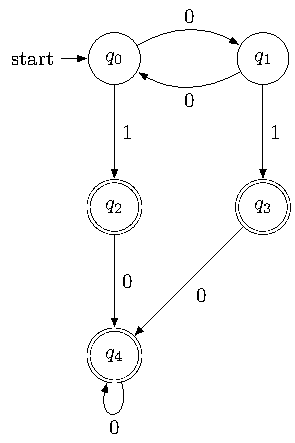
\includegraphics[width=\textwidth]{automaton_4_1}
        \caption{}
        \label{fig:DFA4_1}
    \end{subfigure}
    \\
    \begin{subfigure}[b]{0.35\textwidth}
        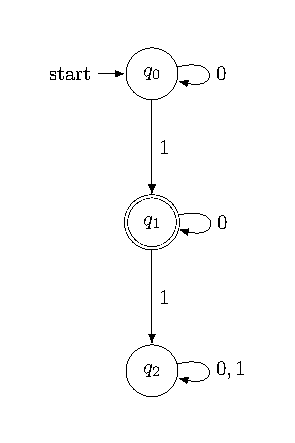
\includegraphics[width=\textwidth]{automaton_4_2}
        \caption{}
        \label{fig:DFA4_2}
    \end{subfigure}
    ~
    \begin{subfigure}[b]{0.35\textwidth}
        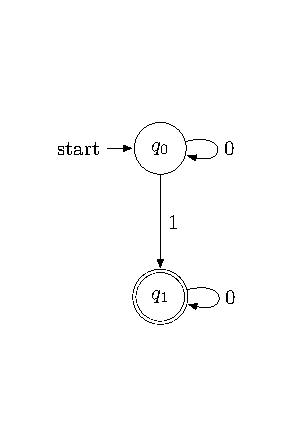
\includegraphics[width=\textwidth]{automaton_4_3}
        \caption{}
        \label{fig:DFA4_3}
    \end{subfigure}
    \caption{(a)接受{$\mathcal{L}$}=0*10*的自动机{\cite[fig 5-4]{book1}};  (b) 图(a)去除非 “final-reachable” 状态 {$q_5$}; (c) 与图(a) 的 $DFA$ 同构的含有陷阱状态的最小 $DFA$ ;(d) 与图(a) 的 $DFA$ 同构的不含陷阱状态的最小 $DFA$。}
    \label{fig:DFA4}
\end{figure}



\begin{figure}[!htbp]
    \centering
    \begin{subfigure}[b]{0.3\textwidth}
        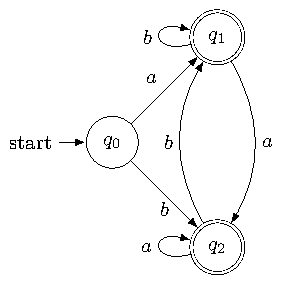
\includegraphics[width=\textwidth]{Min/DFAMinTest-3-0}
        \caption{}
        \label{fig:DFAMin-3-0}
    \end{subfigure}
    ~
    \begin{subfigure}[b]{0.3\textwidth}
        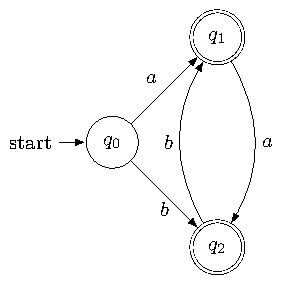
\includegraphics[width=\textwidth]{Min/DFAMinTest-3-1}
        \caption{}
        \label{fig:DFAMin-3-1}
    \end{subfigure}
    ~
    \begin{subfigure}[b]{0.3\textwidth}
        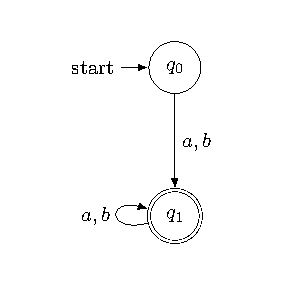
\includegraphics[width=\textwidth]{Min/DFAMinTest-3-2}
        \caption{}
        \label{fig:DFAMin-3-2}
    \end{subfigure}
    \caption{(a)一个 DFA; (b) 图(a)去除转移关系$T=\{(1 \times \mbox{'b'} \times 1),(2 \times \mbox{'a'} \times 2)\}$ 后的最小的 DFA ; (c) 与图(a) 同构的最小的 DFA }
    \label{fig:DFAMin-3}
  \end{figure}

  \begin{figure}[!htbp]
    \centering
    \begin{subfigure}[b]{0.9\textwidth}
        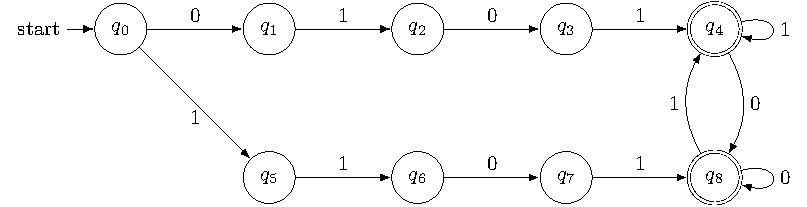
\includegraphics[width=\textwidth]{Min/DFAMinTest-5-0}
        \caption{}
        \label{fig:DFAMin-5-0}
    \end{subfigure}
    \\
    \begin{subfigure}[b]{0.9\textwidth}
        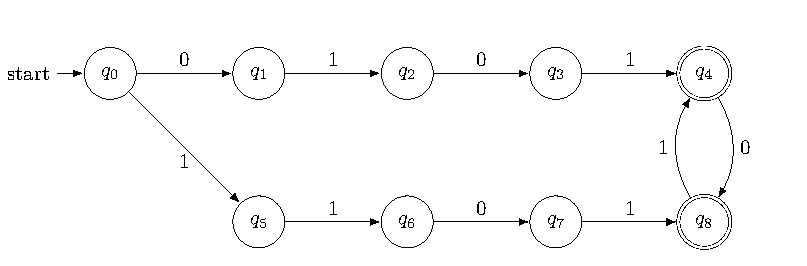
\includegraphics[width=\textwidth]{Min/DFAMinTest-5-1}
        \caption{}
        \label{fig:DFAMin-5-1}
    \end{subfigure}
    \\
    \begin{subfigure}[b]{0.9\textwidth}
        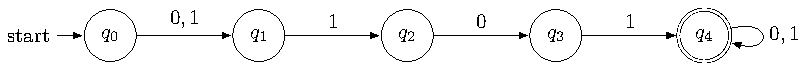
\includegraphics[width=\textwidth]{Min/DFAMinTest-5-2}
        \caption{}
        \label{fig:DFAMin-5-2}
    \end{subfigure}
    \caption{(a)一个 DFA; (b) 图(a)去除转移关系$T=\{(4 \times \mbox{'1'} \times 4),( 8 \times \mbox{'0'} \times 8 )\}$ 后的最小的 DFA ; (c) 与图(a) 同构的最小的 DFA }
    \label{fig:DFAMin-5}
  \end{figure}


  \begin{figure}[!htbp]
    \centering
    \begin{subfigure}[b]{0.7\textwidth}
        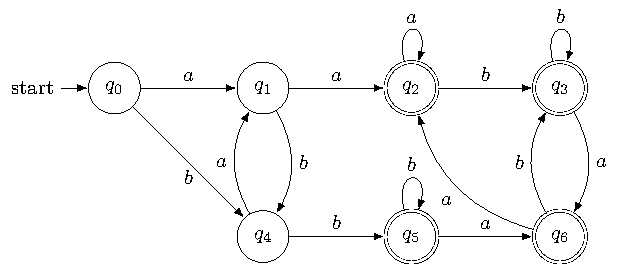
\includegraphics[width=\textwidth]{Min/DFAMinTest-4-0}
        \caption{}
        \label{fig:DFAMin-4-0}
    \end{subfigure}
    \\
    \begin{subfigure}[b]{0.7\textwidth}
        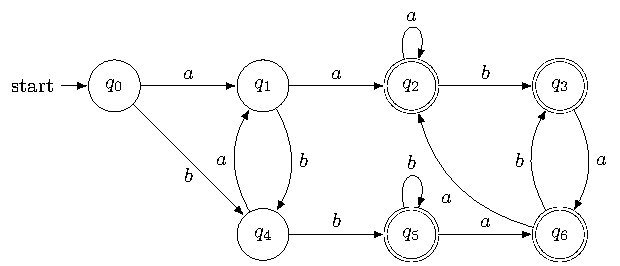
\includegraphics[width=\textwidth]{Min/DFAMinTest-4-1}
        \caption{}
        \label{fig:DFAMin-4-1}
    \end{subfigure}
    \\
    \begin{subfigure}[b]{0.7\textwidth}
        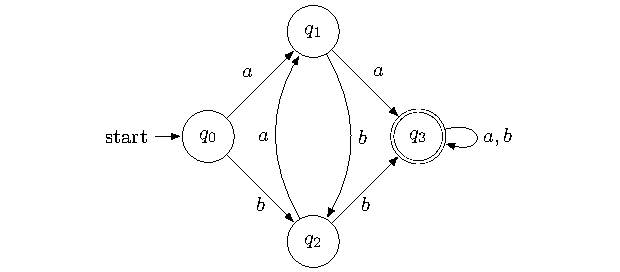
\includegraphics[width=\textwidth]{Min/DFAMinTest-4-2}
        \caption{}
        \label{fig:DFAMin-4-2}
    \end{subfigure}
    \caption{(a)一个 DFA; (b) 图(a)去除转移关系$T=\{(3 \times \mbox{'b'} \times 3)\}$ 后的最小的 DFA ; (c) 与图(a) 同构的最小的 DFA }
    \label{fig:DFAMin-4}
  \end{figure}

\begin{figure}[!htbp]
  \centering
  \begin{subfigure}[b]{0.35\textwidth}
      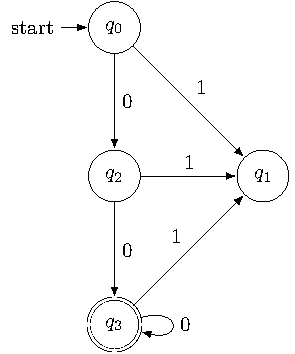
\includegraphics[width=\textwidth]{usefulf2-1}
      \caption{}
      \label{fig:usefulf2-1}
  \end{subfigure}
  ~
  \begin{subfigure}[b]{0.35\textwidth}
      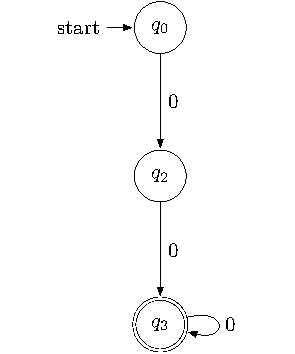
\includegraphics[width=\textwidth]{usefulf2-2}
      \caption{}
      \label{fig:usefulf2-2}
  \end{subfigure}
  \caption{(a)接受{$\mathcal{L}$}=000*的最小的 DFA;  (b) 图(a)去除非 “final-reachable” 状态 {$q_1$}; }
  \label{fig:usefulf2-0}
\end{figure}




\begin{figure}[!htbp]
    \centering
    \begin{subfigure}[b]{0.7\textwidth}
        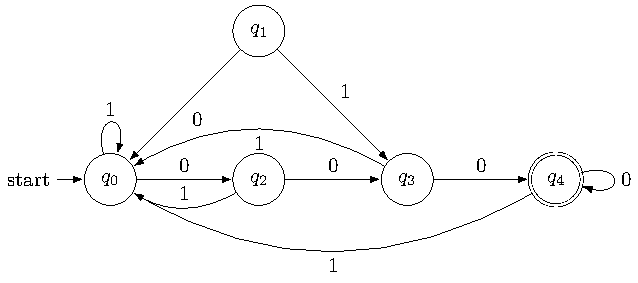
\includegraphics[width=\textwidth]{keepMin/mindfa1-with-start-unreachable}
        \caption{}
        \label{fig:keepMin-1-unreachable}
    \end{subfigure}
    \\
    \begin{subfigure}[b]{0.7\textwidth}
        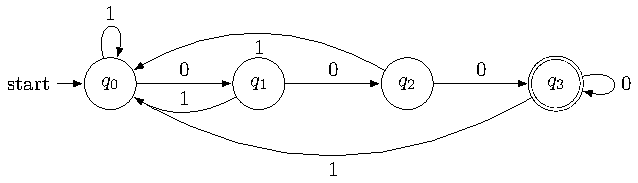
\includegraphics[width=\textwidth]{keepMin/mindfa1}
        \caption{}
        \label{fig:keepMin-1-nonTheState}
    \end{subfigure}
    \caption{(a)接受{$\mathcal{L}=\{ x000 | x \in \{ 0,1\}^{*} \}$}的最小的 DFA;  (b) 图(a)去除开始不可达状态 {$q_1$}; }
    \label{fig:keepMin-1}
\end{figure}

\begin{figure}[!htbp]
    \centering
    \begin{subfigure}[b]{0.7\textwidth}
        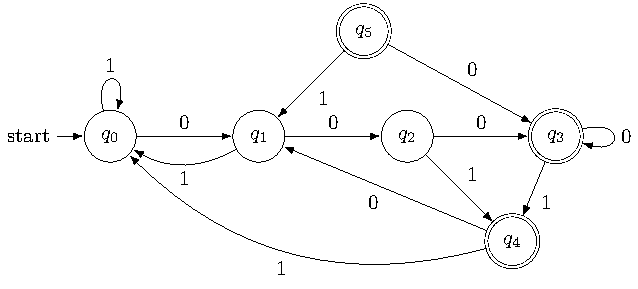
\includegraphics[width=\textwidth]{keepMin/mindfa2-with-start-unreachable}
        \caption{}
        \label{fig:keepMin-2-unreachable}
    \end{subfigure}
    \\
    \begin{subfigure}[b]{0.7\textwidth}
        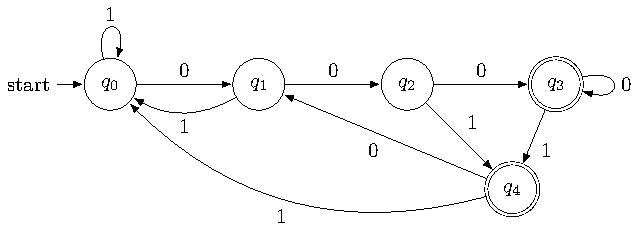
\includegraphics[width=\textwidth]{keepMin/mindfa2}
        \caption{}
        \label{fig:keepMin-2-nonTheState}
    \end{subfigure}
    \caption{(a)接受{$\mathcal{L}=\{ x000 | x \in \{ 0,1\}^{*} \cup \{ x001 | x \in \{ 0,1\}^{*} \}$}的最小的 DFA;  (b) 图(a)去除开始不可达状态 {$q_5$}; }
    \label{fig:keepMin-2}
\end{figure}


\begin{figure}[!htbp]
    \centering
    \begin{subfigure}[b]{0.49\textwidth}
        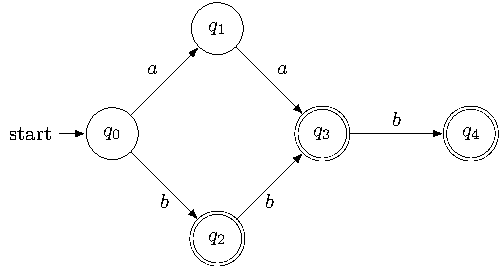
\includegraphics[width=\textwidth]{keepMin/hoperror--1}
        \caption{$\mathcal{L}=\{aa \cup aab \cup b \cup bb \cup bbb\}$}
        \label{fig:hoperror--1}
    \end{subfigure}
    ~
    \begin{subfigure}[b]{0.49\textwidth}
        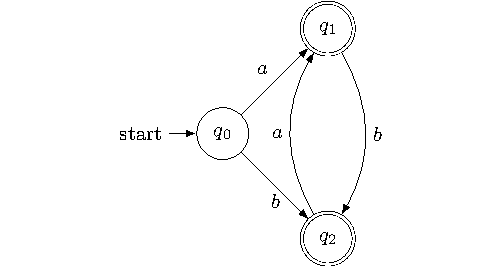
\includegraphics[width=\textwidth]{keepMin/hoperror--2}
        \caption{}
        \label{fig:hoperror--2}
    \end{subfigure}
    \\
    \begin{subfigure}[b]{0.7\textwidth}
        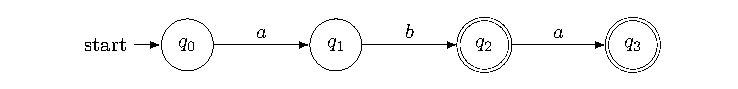
\includegraphics[width=\textwidth]{keepMin/hoperror--3}
        \caption{$\mathcal{L}=\{ab \cup aba\}$}
        \label{fig:hoperror--3}
    \end{subfigure}
    ~
    \begin{subfigure}[b]{0.7\textwidth}
        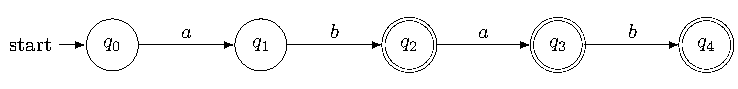
\includegraphics[width=\textwidth]{keepMin/hoperror--4}
        \caption{$\mathcal{L}=\{ab \cup aba \cup abab\}$}
        \label{fig:hoperror--4}
    \end{subfigure}
    ~
    \begin{subfigure}[b]{0.7\textwidth}
        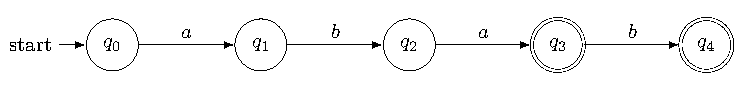
\includegraphics[width=\textwidth]{keepMin/hoperror--5}
        \caption{$\mathcal{L}=\{aba \cup abab\}$}
        \label{fig:hoperror--5}
    \end{subfigure}
    \caption{一组最小的 DFA }
    \label{fig:hopcerror}
  \end{figure}

\begin{figure}[!htbp]
    \centering
    \begin{subfigure}[b]{0.9\textwidth}
        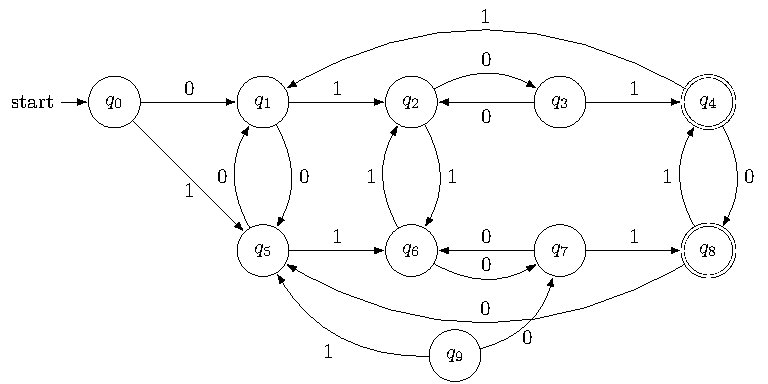
\includegraphics[width=\textwidth]{DFA11-0}
        \caption{}
        \label{fig:DFA11-0}
    \end{subfigure}
    \\
    \begin{subfigure}[b]{0.9\textwidth}
        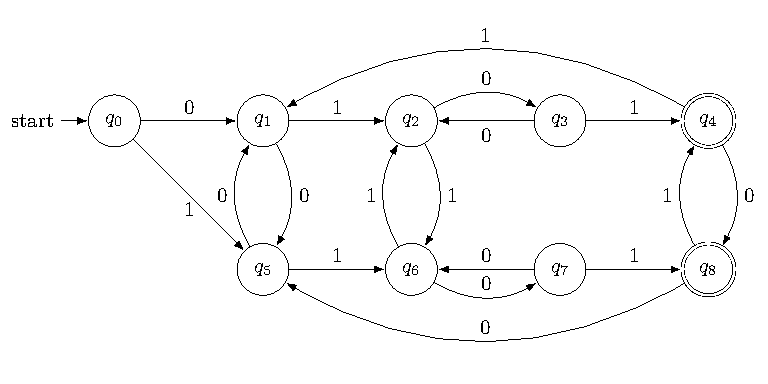
\includegraphics[width=\textwidth]{DFA11-1}
        \caption{}
        \label{fig:DFA11-1}
    \end{subfigure}
    \\
    \begin{subfigure}[b]{0.9\textwidth}
        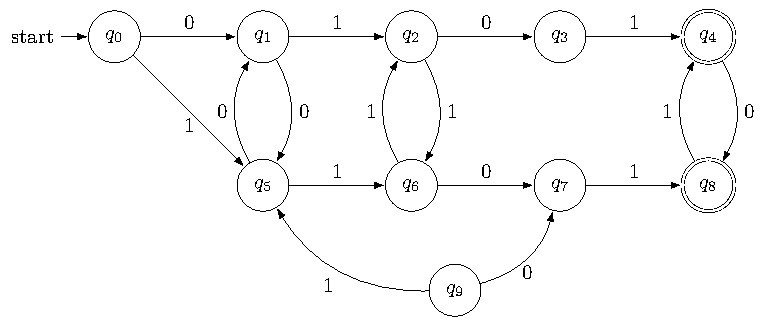
\includegraphics[width=\textwidth]{DFA11-2}
        \caption{}
        \label{fig:DFA11-2}
    \end{subfigure}
    \caption{(a)一个最小的DFA;  (b) 图(a) 移除开始不可达状态 {$q_9$};(c) 图(a)移除转移关系$T=\{(4 \times '1' \times 1),(8 \times '0' \times 5),(3 \times '0' \times 2),(7 \times '0' \times 6)\}$后的DFA。 }
    \label{fig:DFA11}
  \end{figure}